% ---- Modele TP PC V2 -----------
\documentclass[a4paper,10pt,french]{scrartcl}
\usepackage[T1]{fontenc}%---pour l'encodage d'entr\'ee
\usepackage{array}%---pour les tableaux
\usepackage{titlesec}%---modification des titres
\usepackage{ulem}%---pour le soulignage
\usepackage[dvipsnames]{xcolor}%---pour avoir d'autres couleurs
\usepackage{color}%---pour avoir les couleurs de base
\usepackage{babel}%---pour les trucs de langue et la francisation

\usepackage{graphicx}%----pour mettre des images
\usepackage[utf8]{inputenc}%---encodage
\usepackage{geometry}%---pour modifier les tailles et mettre a4paper
%\usepackage{awesomebox}%---pour les boites d'exercices, de pbq et de croquis ---d\'esactiv\'e pour les TP de PC
\usepackage{tikz}%---pour dessiner + d\'ependance de chemfig
%\usepackage{tabularx}%---pour dimensionner automatiquement les tableaux avec variable X
\usepackage{fancyhdr}%---pour les en-t\^ete personnalis\'ees
\usepackage{blindtext}%---pour les liens
\usepackage{hyperref}%---pour les liens (\`a mettre en dernier)
\usepackage{caption}%---pour la francisation de la l\'egende table vers Tableau
 \usepackage{float}% --- pour placer les figures et tableaux où l'on souhaite avec argument H
 \usepackage{multicol}
 \usepackage{amsmath}
 \usepackage{geometry}
 %\geometry{vmargin=2.5cm}

\captionsetup{labelfont=sc}%---pour la francisation de la l\'egende table vers Tableau
\def\frenchtablename{Tableau}%---pour la francisation de la l\'egende table vers Tableau
\pagestyle{fancy}
\renewcommand\headrulewidth{1pt}
\fancyhead[L]{TP 3}
\fancyhead[R]{Saux Paulhenry}
\title{Compte rendu de TP 3}
\date{}
\author{}

\geometry{a4paper}
% ----------- Création des commandes de couleur ----------
\makeatletter
\newcommand{\coloruline}[2]{%
        \UL@protected\def\temp@uline{\leavevmode \bgroup
            \markoverwith{\textcolor{#1}{\rule[-0.5ex]{2pt}{0.4pt}}}%
        \ULon}%
        \temp@uline{#2}%
    }

    \newcommand{\coloruuline}[2]{%
        \UL@protected\def\temp@uuline{\leavevmode \bgroup
            \UL@setULdepth
            \ifx\UL@on\UL@onin \advance\ULdepth2.8\p@\fi
            \markoverwith{\textcolor{#1}{\lower\ULdepth\hbox
                {\kern-.03em\vbox{\hrule width.2em\kern1\p@\hrule}\kern-.03em}}}%
        \ULon}%
        \temp@uuline{#2}%
    }

\makeatother

\renewcommand{\thesection}{\arabic{section}}
\renewcommand{\thesubsection}{\arabic{subsection}}
\renewcommand{\thesubsubsection}{\arabic{subsubsection}}
\begin{document}
% ---------------- Modification des titres de niveau 1,2 et 3 --------------------
\titleformat
{\section} % command
%[display] % shape
{\Large} % format
{\coloruuline{red}{\thesection. }} % label
{0ex} % sep
{\coloruuline{red}} % before-code
[] % after-code

\titleformat
{\paragraph} % command
%[display] % shape
{\Large} % format
{\coloruline{NavyBlue}{\theparagraph. }} % label
{0ex} % sep
{\coloruline{NavyBlue}} % before-code
[] % after-code

\titleformat
{\subsection} % command
%[display] % shape
{\Large} % format
{\coloruline{red}{\thesection.\thesubsection. }} % label
{0ex} % sep
{\coloruline{red}} % before-code
[] % after-code

\titleformat
{\subsubsection} % command
%[display] % shape
{\large} % format
{\coloruline{ForestGreen}{\thesection.\thesubsection.\thesubsubsection. }} % label
{0ex} % sep
{\coloruline{ForestGreen}} % before-code
[] % after-code

\titleformat
{\chapter} % command
%[display] % shape
{\large} % format
{\coloruline{NavyBlue}{\thechapter \:- }} % label
{0ex} % sep
{\coloruline{NavyBlue}} % before-code
[] % after-code


% ---------------- Début du corps du document ------------------------------------

\section{Introduction}
\subsection{Objectifs}
L'objectif de ce TP est de mettre en évidence les propriétés optiques fondamentales des réseaux optiques. Pour cela, nous étudirons le spectre et figures de diffractions obtenus à partir d'une lampe à mercure.
\subsection{Sommaire}
Ce TP se décompose en quatre parties :
\begin{enumerate}
 \item Réglage du goniomètre
 \item Étude du réseau en incidence normale
 \item Étude du réseau en incidence variable
 \item Étude du minimum de déviation du réseau
\end{enumerate}
\section{Protocole}
\subsection{Matériel}
\begin{itemize}
\item Réseau d'amplitude en transmission
\item Lampe à vapeur de mercure
\item Goniomètre de précision
\end{itemize}
\subsection{Description du montage expérimental}
Le goniomètre est composé d'une lunnette, d'une platine sur lequel se trouve le réseau et d'une lentille collimateur. La lunette se compose d'un occulaire, d'une source de lumière accompagnée d'un miroir escamotable, d'un réticule et d'une lentille objectif. Une représentation schématique se trouve en figure 1


\begin{figure}[H]
 \begin{center}
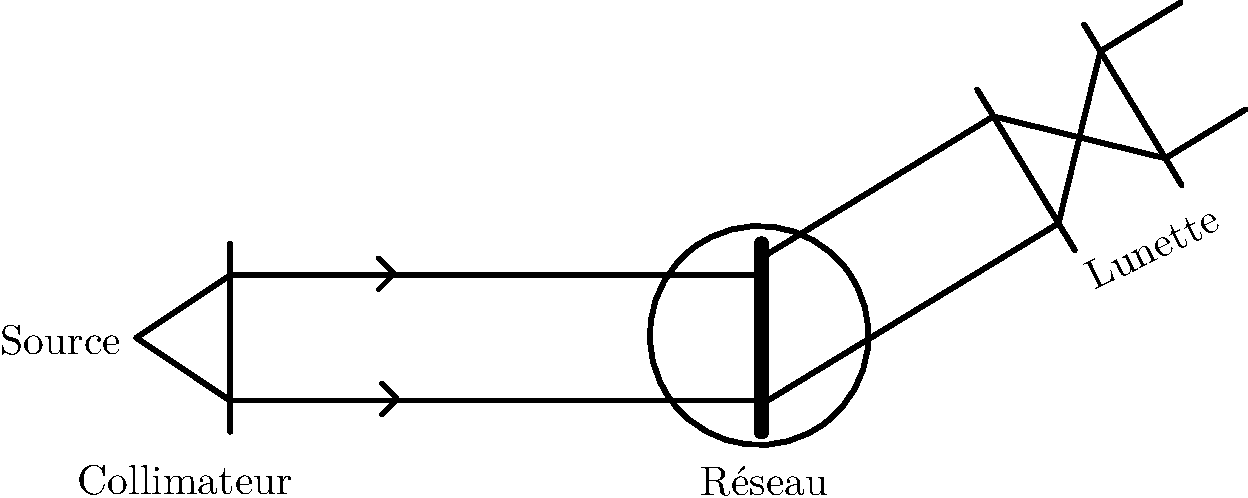
\includegraphics[scale=0.5]{goniometre}
 \end{center}
\caption{Schéma représentant le trajet de la mumière dans le goniomètre}
\end{figure}


\begin{center}
%
\includegraphics[scale=0.3]{circuit1}
\end{center}
\subsection{Réglages}
\subsubsection{Lunette}
Le réglage se divise en 2 parties : l'une fixe et l'autre qui dépend de la vue de l'observateur. On commencer par le réglage de l'occulaire, qui dépend de l'observateur. Pour cela, on ajuste simplement la distance entre le réticule et l'occulaire.

Le deuxième réglalge permet d'oberser une image nette quand les faiseaux proviennent de l'infini. Pour cela, on utilise le miroir escamotable pour observer par la méthode d'autocollimation l'image nette du réticule.
\subsubsection{Collimateur}
Le but de ce réglage est d'obtenir en entré du réseau des rayons parallèles. On ajuste pour cela la distance entre la fente source et la lentille du collimateur.
\subsubsection{Relève du décalage par rapport au 0}
Il faut maintenant relever la valeur de décalage par rapport 0. En effet, le zéro du cercle gradué n’est pas forcément aligné avec la direction réelle du faisceau. Cette valeur est la normale initiale au réseau et sera notée \(\Theta_{i,0}\).
\subsection{Mesures à effectuer}
\subsubsection{Étude en incidence normale}
\begin{enumerate}
 \item La lunette se trouve en position \(\Theta_{i,0}\)
 \item On active le miroir escamotable de la lunette
 \item On fait pivoter le réseau de façon à faire coincider le réticule de la lunette et on image par le réseau.
 \item Relever les positions des angles pour différentes raies (violet, indigo, bleu-vert, vert, doublet jaune) en se déplaçant dans le sens antitrigonométrique (voir schéma).
\end{enumerate}
\subsubsection{Étude en incidence variable}
\begin{enumerate}
 \item La lunette se trouve en position \(\Theta_{i,0}\)
 \item Régler la lunette sur l'angle \(\theta_i\)
 \item Faire pivoter le réseau de façon à faire coincider le réticule de la lunette et on image par le réseau.
 \item Replacer la lunette en \(\Theta_{i,0}\)
 \item Relever l'angle pour la raie de couleur verte en déplaçant dans le sens antitrigonométrique. Il faudra soustraire à l'angle relevé l'angle \(\theta_i\).
\end{enumerate}
\subsection{Étude du minimum de déviation}
\begin{enumerate}
 \item  La lunette se trouve en position \(\Theta_{i,0}\)
 \item Avec une feuille blanche, relever la position de la raie verte
 \item Faire tourner le réseau dans le sens trigonométrique et suivre avec la feuille la raie
 \item Une fois que la raie ne parvent plus à ce décaler vers l'extérieur, relever avec le vernier la position de la raie
 \item Faire de m\^eme dans le sens antitrigonométrique.
\end{enumerate}

\section{Mesures}
\subsection{Étude en incidence normale}
\subsubsection{Données}
\begin{center}
\begin{tabular}{llll}
Raie & Longueur d’onde & Angle Brut & Angle par rapport à la normale\\
Jaune & 579 & 200,07 & 19,99\\
Jaune 2 & 577 & 200,02 & 19,94\\
Vert & 546,1 & 198,56 & 18,48\\
Bleu-vert & 491,6 & 197,0 & 16,92\\
Indigo & 435,8 & 195 & 14,92\\
Violet & 404,7 & 193,57 & 13,49
\end{tabular}
\end{center}

\subsubsection{Incertitudes}
L'incertitude du goniomètre est de 30'', une fois bien réglé. La position du réticule sur notre goniomètre n'étant pas optimale (trop bas pour une lecture précise), on ajoute neviron 1' à l'incertitude due à l'imprecision du réglage. De plus, de par la largeur des raies, on peut ajouter environ 10'', ce qui donne une incertitude de \(1,40'\) environ.
\subsection{Étude en incidence variable}
\subsubsection{Données}
Ici, le décalage par rapport au 0 est de 180.8.
\begin{center}
\begin{tabular}{lllll}
\(\theta_i\) & \(\theta_{if}\) & \(\theta_d\) & \(\theta_{df}\) & \(\theta_{df,c}\)\\
10 & 190 & 198,4 & 8,4 & -8.4\\
20 & 200 & 199 & -1\\
30 & 210 & 199,53 & -10,47 & 10,47\\
40 & 220 & 201,24 & -18,76 & 18,76\\
50 & 230 & 203,44 & -26,56 & 26,56\\
60 & 240 & 207,08 & -32,92 & 32,92
\end{tabular}
\end{center}
Les angles \(\theta_{df,c}\) sont obtnus en prenant l'opposé des angles mesurés pour respecter les conventions du sens positif dans les parties théoriques, qui sont différentes de celles présentes dans la manipulation.
\subsubsection{Incertitudes}
L'incertitude sur la différence vaut 2 fois l'incertitude du goniomètre soit \(60''\).
\subsection{Étude au minimum de déviation}
\subsubsection{Données}
\begin{center}
\begin{tabular}{ll}
Angle minium 1 & Angle miniumum 2\\
199.52 & 161.35
\end{tabular}
\end{center}

\section{Graphiques}
\subsection{Étude en incidence normale}
\begin{figure}[H]
 \begin{center}
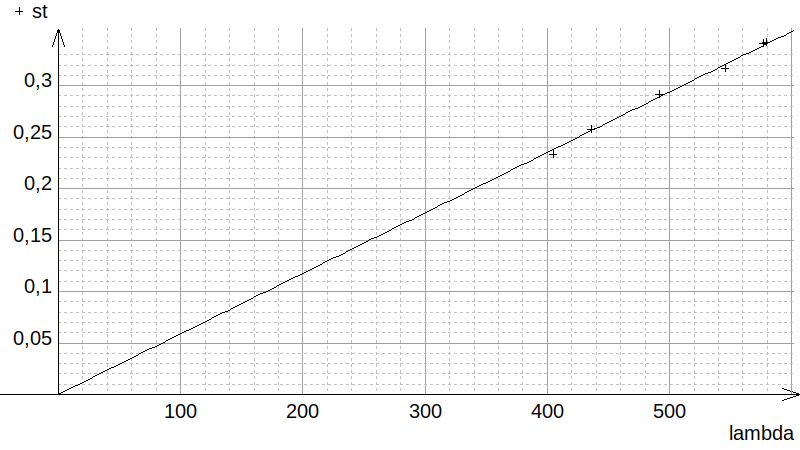
\includegraphics[scale=0.45]{tp_optique_3}
 \end{center}
\caption{Évolution de \(\sin(\theta_d)\) en fonction de la longueur d'onde de la raie \(\cdot 10^{-9}\)m}
\end{figure}
\subsection{Étude en incidence variable}
\begin{figure}[H]
 \begin{center}
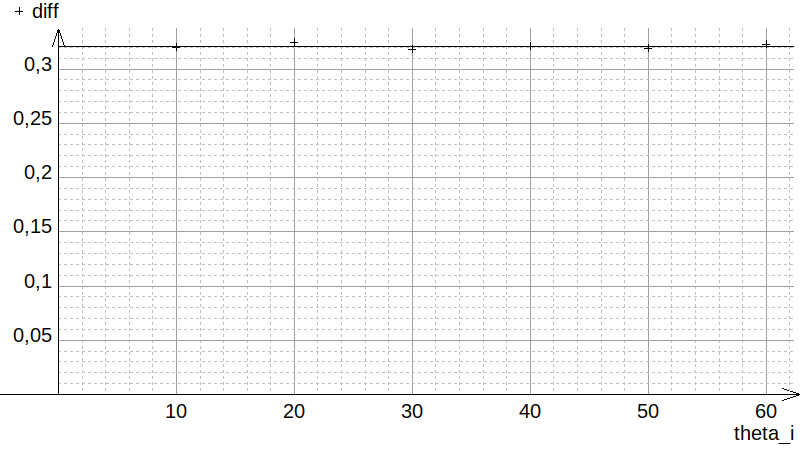
\includegraphics[scale=0.45]{tp_optique_3_2}
 \end{center}
\caption{Évolution de \(\sin(\theta_d)-\sin(\theta_i)\) en fonction de \(\theta_i\) (°)}
\end{figure}
\section{Exploitation des résultats}
\subsection{Étude en incidence normale}
On utilise la relation
\begin{equation}
 \sin(\theta_d)-\sin(\theta_i)=kN\lambda = k\lambda\frac{1}{p}
\end{equation}


Avec regressi, on obtient en traçant \(\sin(\theta_d) =f(\lambda)\) et en modélisant par \(\sin(\theta_d) = N\times \lambda\) les valeurs \(N = (587,5\pm 2,5)10^{3}m^{-1}\) et \(p= (1,7022 \pm0,0073)10^{-3}\)m.

On peut aussi retrouver ces valeurs en utilisant la relation indivduellement sur chaque mesure à l'aide de la formule ci-dessus, en posant \(\sin(\theta_i) = 0 \) car nous sommes en incidence normale.

L'incertitude liée à la longueur d'onde peut \^etre négligée devant celle liée à la mesure de l'angle. Celle ci-dépend de l'angle brut et de l'angle de la normale mesuré. L'incertutide sur un angle doit donc \^etre multipliée par 2. On obtient finalement \(u(\theta_d)= 2.8'\simeq 0.05°\). On peut déterminer l'incertitude sur les résultats avec \(u(N) = N\cdot\frac{u(\theta_d)}{\theta_d}\). De cette façon, on obtient finalement :
\begin{center}
\begin{tabular}{llll}
Raie & Longueur d’onde (\(\cdot 10^{-9}m\)) & N calculé (\(\cdot 10^{3}m^{-1}\)) & Incertitude (\(\cdot 10^{3}m^{-1}\))\\
Jaune & 579 & 590,1 & 1,4\\
Jaune 2 & 577 & 590,7 & 1,4\\
Vert & 546,1 & 580,1 & 1,5\\
Bleu-vert & 491,6 & 591,7 & 1,7\\
Indigo & 435,8 & 590,5 & 1,9\\
Violet & 404,7 & 576,1 & 2,1
\end{tabular}
\end{center}
\subsection{Étude en incidence variable}
Nous avons mesuré en réalité à chaque fois la raie de l'ordre -1, nous devons donc, pour obtenir une égalité avec \(\lambda \cdot N\), multiplier par \(-1\). De cette façon, on obtient
\begin{center}
\begin{tabular}{lll}
\(theta_i\) & \(theta_d\) & \(\sin(\theta_d)-\sin(\theta_i)\)\\
10 & -8,4 & 0,319570542099958\\
20 & 1 & 0,324410288837497\\
30 & 10,47 & 0,31814053087621\\
40 & 18,76 & 0,321068893728363\\
50 & 26,56 & 0,318835471511551\\
60 & 32,92 & 0,322536871163414
\end{tabular}
\end{center}
En modélisant dans régressi, on obtient une nouvelle valeur de N : \(N = N=(587,5 \pm1,8)10^{3} \). On remarque que l'incertitude sur ce résultat est plus faible que pour le résultat précédent.

On peut aussi trouver des résultats semblables en effectuant le calcul pour des mesures individuelles. L'incertitude sur le résultat est lié à l'incertitude de \(\theta_i\) et \(\theta_d\).

On utilise donc la formule : \[\frac{u(N)}{N} = \sqrt{(\frac{u(\theta_d)}{\theta_d})^2 + (\frac{u(\theta_i)}{\theta_i})^2}\]

Les incertitudes sur \(\theta_i\) et \(\theta_d\) sont aussi de \(2.8'\) chacunes.


Par exemple, pour la mesure $\theta_i = 30^\circ$ et $\theta_d = 10{,}47^\circ$, l'incertitude angulaire vaut

\[
u(\theta) = 2.8' = \frac{2.8}{60}^\circ = 0.04667^\circ.
\]
Les incertitudes relatives sont alors :
\[
\frac{u(\theta_i)}{\theta_i} = \frac{0.04667}{30} = 1.56\times 10^{-3}, \qquad
\frac{u(\theta_d)}{\theta_d} = \frac{0.04667}{10.47} = 4.46\times 10^{-3}.
\]
L'incertitude relative sur $N$ devient :
\[
\frac{u(N)}{N}
= \sqrt{(4.46\times 10^{-3})^2 + (1.56\times 10^{-3})^2}
= 4.72\times 10^{-3}.
\]
En prenant $N = 5.87\times 10^{5}$, on obtient :
\[
u(N) = 5.87\times 10^{5} \times 4.72\times 10^{-3}
      = 2.77\times 10^{3}
\]
Ainsi,
\[
N = (5.87 \pm 0.28)\times 10^{5}
\]
L'incertitude est nettement plus grande que celle obtenue par régression, ce qui est normal (et attendu) : la régression linéaire réduit l’incertitude en combinant plusieurs mesures.
\subsection{Minium de déviation}
On peut calculer le minimum de déviation avec
\begin{equation}
 D_m = \frac{Y_1-Y_2}{2}
\end{equation}
On en déduit N avec
\begin{equation}
 2\sin(\frac{D_m}{2}) = kN\lambda
\end{equation}
Ici, k=1.

On mesure les angles $Y_1$ et $Y_2$ avec les mêmes incertitudes $u(Y_1) = u(Y_2) = u(Y)$.

Le minimum de déviation est
\[
D_m = \frac{Y_1 - Y_2}{2}.
\]

Ce qui correspond à une incertitude de
\[
u(D_m) = \frac{1}{2}\sqrt{u(Y_1)^2 + u(Y_2)^2}
       = \frac{1}{2}\sqrt{2\,u(Y)^2}
       = \frac{u(Y)}{\sqrt{2}}.
\]

Si l’on suppose $\lambda$ sans incertitude et que l’angle est suffisamment petit\footnote{On suppose que l'angle trouvé, d'environ 15° est assez petit pour réaliser l'approximation.} pour approximer
\[
\sin\left(\frac{D_m}{2}\right) \approx \frac{D_m}{2},
\]
on obtient alors
\[
N \approx \frac{D_m}{\lambda}.
\]

Dans ce cas, on a
\[
\frac{u(N)}{N} = \frac{u(D_m)}{D_m}.
\]

En remplaçant $u(D_m)$, on obtient
\[
\frac{u(N)}{N} = \frac{u(Y)}{\sqrt{2}\,D_m}
\]
et
\[
u(N) = N \,\frac{u(Y)}{\sqrt{2}\,D_m}.
\]

En prenant \(u(Y) = 1.4'\) et les valeurs obtenues de Y, on obtient finalement \(N=(6.07\pm0.05)\cdot10^5 m^{-1}\). C'est proche des valeurs obtenues en partie précédente.
\section{Conclusion}
Ce TP nous a permis d'appréhender les propriétés de diffraction d'un réseau optique en utilisant les raies d'émission d'une lampe à vapeur de mercure. Nous avons pu déterminer la densité de traits $N$ à l'aide de 3 approches :
\begin{itemize}
    \item L'étude en incidence normale, exploitée par régression linéaire, nous a permis d'obtenir une valeur de $N = (587,5 \pm 2,5) \cdot 10^{3} \, \text{m}^{-1}$.
    \item L'étude en incidence variable, également exploitée par régression linéaire, a abouti à une valeur cohérente de $N = (587,5 \pm 1,8) \cdot 10^{3} \, \text{m}^{-1}$, présentant l'incertitude la plus faible grâce à la multiplication des points de mesure.
    \item Enfin, la méthode du minimum de déviation a donné un résultat de $N = (607 \pm 5) \cdot 10^{5} \, \text{m}^{-1}$.
\end{itemize}

L'écart observé avec la méthode du minimum de déviation peut s'expliquer la difficulté expérimentale à identifier avec précision le point de rebroussement de la raie verte. De plus, contrairement aux autres méthodes, nous ne pouvons pas réduire l'erreur en faisant plusieurs mesures pour la m\^eme raie\footnote{On aurait pu cependant effectuer la mesure du mimum de déviation avec d'autres raies puis effectuer, comme avec les autres méthodes, une regression linéaire pour déterminer N}.

Néanmoins, la convergence des résultats obtenus en incidence normale et variable valide la loi des réseaux : $\sin(\theta_d) - \sin(\theta_i) = kN\lambda$. Ce travail met en évidence l'importance cruciale des réglages préliminaires du goniomètre (autocollimation et réglage du collimateur) pour minimiser les erreurs systématiques et garantir la fiabilité des mesures angulaires.


L'indication fournie pour le réseau est de $15\,000$ traits par pouce. Comme un pouce correspond à  $0,0254$ m, la densité de traits théorique $N_{th}$ est :
\[
N_{th} = \frac{15\,000}{0,0254} \approx 590\,551 \text{ m}^{-1} \approx 590,6 \cdot 10^3 \text{ m}^{-1}
\]

Nous avons obtenu expérimentalement $N_{exp} = (587,5 \pm 2,5) \cdot 10^3 \text{ m}^{-1}$. L'erreur relative entre la valeur théorique et la valeur expérimentale est de :
\[
\frac{|N_{th} - N_{exp}|}{N_{th}} = \frac{|590,6 - 587,5|}{590,6} \approx 0,52\%
\]

Cet écart très faible confirme la validité de nos mesures. La légère différence peut s'expliquer par l'imprécision du réglage du goniomètre.
\end{document}
